%-----------------------------------------------------------------------
% Cgins: Incompressible Navier Stokes Solver
%        REFERENCE MANUAL
%-----------------------------------------------------------------------
\documentclass[10pt]{article}
% \usepackage[bookmarks=true]{hyperref}  % this changes the page location !
\usepackage[bookmarks=true,colorlinks=true,linkcolor=blue]{hyperref}

% \input documentationPageSize.tex
\hbadness=10000 
\sloppy \hfuzz=30pt

% \voffset=-.25truein
% \hoffset=-1.25truein
% \setlength{\textwidth}{7in}      % page width
% \setlength{\textheight}{9.5in}    % page height

\usepackage{calc}
\usepackage[lmargin=.75in,rmargin=.75in,tmargin=.75in,bmargin=.75in]{geometry}

% \input homeHenshaw

% \input{pstricks}\input{pst-node}
% \input{colours}
\newcommand{\blue}{\color{blue}}
\newcommand{\green}{\color{green}}
\newcommand{\red}{\color{red}}
\newcommand{\black}{\color{black}}


\usepackage{amsmath}
\usepackage{amssymb}

\usepackage{verbatim}
\usepackage{moreverb}

\usepackage{graphics}    
\usepackage{epsfig}    
\usepackage{calc}
\usepackage{ifthen}
\usepackage{float}
% the next one cause the table of contents to disappear!
% * \usepackage{fancybox}

\usepackage{makeidx} % index
\makeindex
\newcommand{\Index}[1]{#1\index{#1}}

\usepackage{tikz}
\usepackage{pgfplots}
\input ../common/trimFig.tex


% ---- we have lemmas and theorems in this paper ----
\newtheorem{assumption}{Assumption}
\newtheorem{definition}{Definition}

% \newcommand{\homeHenshaw}{/home/henshaw.0}

\newcommand{\Overture}{{\bf Over\-ture\ }}
% \newcommand{\ogenDir}{\homeHenshaw/Overture/ogen}

\newcommand{\cgDoc}{../../cgDoc}
\newcommand{\cgDir}{../../cg}
% \newcommand{\vpDir}{\homeHenshaw/overtureFramework/cgDoc/ins/viscoPlastic}

% \newcommand{\ovFigures}{\homeHenshaw/OvertureFigures}
% \newcommand{\obFigures}{\homeHenshaw/res/OverBlown/docFigures}  % for figures
% \newcommand{\convDir}{\homeHenshaw/overtureFramework/cgDoc/ins/tables}
\newcommand{\convDir}{tables}
% \newcommand{\insDocDir}{\homeHenshaw/overtureFramework/cgDoc/ins}
\newcommand{\insDocDir}{.}

% *** See http://www.eng.cam.ac.uk/help/tpl/textprocessing/squeeze.html
% By default, LaTeX doesn't like to fill more than 0.7 of a text page with tables and graphics, nor does it like too many figures per page. This behaviour can be changed by placing lines like the following before \begin{document}

\renewcommand\floatpagefraction{.9}
\renewcommand\topfraction{.9}
\renewcommand\bottomfraction{.9}
\renewcommand\textfraction{.1}   
\setcounter{totalnumber}{50}
\setcounter{topnumber}{50}
\setcounter{bottomnumber}{50}

\begin{document}

\input ../common/wdhDefinitions.tex

\def\comma  {~~~,~~}
\newcommand{\uvd}{\mathbf{U}}
\def\ud     {{    U}}
\def\pd     {{    P}}
\def\calo{{\cal O}}

\newcommand{\mbar}{\bar{m}}
\newcommand{\Rbar}{\bar{R}}
\newcommand{\Ru}{R_u}         % universal gas constant
% \newcommand{\Iv}{{\bf I}}
% \newcommand{\qv}{{\bf q}}
\newcommand{\Div}{\grad\cdot}
\newcommand{\tauv}{\boldsymbol{\tau}}
\newcommand{\thetav}{\boldsymbol{\theta}}
% \newcommand{\omegav}{\mathbf{\omega}}
% \newcommand{\Omegav}{\mathbf{\Omega}}

\newcommand{\Omegav}{\boldsymbol{\Omega}}
\newcommand{\omegav}{\boldsymbol{\omega}}
\newcommand{\sigmav}{\boldsymbol{\sigma}}
\newcommand{\cm}{{\rm cm}}

\newcommand{\ds}{\Delta s}
\newcommand{\dsbl}{\ds_{\rm bl}}


\newcommand{\sumi}{\sum_{i=1}^n}
% \newcommand{\half}{{1\over2}}
\newcommand{\dt}{{\Delta t}}

\def\ff {\tt} % font for fortran variables

% define the clipFig commands:
%% \input clipFig.tex

\newcommand{\Bc}{{\mathcal B}}
\newcommand{\Dc}{{\mathcal D}}
\newcommand{\Ec}{{\mathcal E}}
\newcommand{\Fc}{{\mathcal F}}
\newcommand{\Gc}{{\mathcal G}}
\newcommand{\Hc}{{\mathcal H}}
\newcommand{\Ic}{{\mathcal I}}
\newcommand{\Jc}{{\mathcal J}}
\newcommand{\Lc}{{\mathcal L}}
\newcommand{\Nc}{{\mathcal N}}
\newcommand{\Pc}{{\mathcal P}}
\newcommand{\Rc}{{\mathcal R}}
\newcommand{\Sc}{{\mathcal S}}

\newcommand{\bogus}[1]{}  % removes is argument completely

\vspace{5\baselineskip}
\begin{flushleft}
{\Large
{\bf Cgins} Reference Manual: An Overture Solver for the Incompressible Navier--Stokes Equations on Composite Overlapping Grids, \\
}
\vspace{2\baselineskip}
William D. Henshaw,\\
Department of Mathematical Sciences, \\
Rensselaer Polytechnic Institute, \\
Troy, NY, USA, 12180.
% William D. Henshaw\footnote{This work was performed under the auspices of the U.S. Department of Energy (DOE) by
% Lawrence Livermore National Laboratory under Contract DE-AC52-07NA27344 and by 
% DOE contracts from the ASCR Applied Math Program.}  \\
% Centre for Applied Scientific Computing  \\
% Lawrence Livermore National Laboratory      \\
% Livermore, CA, 94551.  \\
\vspace{\baselineskip}
\today\\
% \vspace{\baselineskip}
% LLNL-SM-455871

\vspace{4\baselineskip}

\noindent{\bf\large Abstract:}

This is the reference guide for {\bf Cgins}.  Cgins is a program that can be
used to solve incompressible fluid flow problems in complex geometry in two and
three dimensions using composite overlapping grids. It is built upon the
\Overture object-oriented framework.  Cgins solves the incompressible
Navier-Stokes equations using a pressure-Poisson formulation. Second-order
accurate and fourth-order accurate approximations are available.
This reference guide describes in some detail the equations being solved,
the discrete approximations, time-stepping methods, boundary conditions and convergence results. 
The reference guide also contains various notes related to different aspects of the equations. 
The reference guide concludes by providing a collection of interesting computations that
have been performed with Cgins. 



% This document describes {\bf Cgins}, a solver written using the \Overture framework
% to solve the incompressible Navier-Stokes (INS).  
% Cgins can be used to the solve time-dependent Navier-Stokes equations to
% second and fourth-order accuracy. There is also a pseudo-steady line implicit solver with
% a nonlinear second- or fourth-order artificial dissipation.

\end{flushleft}

\clearpage
\tableofcontents
% \listoffigures

\vfill\eject


\section{Introduction}

This is the reference guide for {\bf Cgins}.  Cgins is a program that can be
used to solve incompressible fluid flow problems in complex geometry in two and
three dimensions using composite overlapping grids. It is built upon the
\Overture object-oriented framework~\cite{Brown97},\cite{Henshaw96a},\cite{iscope97}.  Cgins solves the incompressible
Navier-Stokes equations using a pressure-Poisson formulation. Second-order
accurate and fourth-order accurate approximations are available.
Cgins can be used to
\begin{itemize}
  \item solve problems in two and three dimensional complex domains,
  \item solve problems on moving grids (specified motion and rigid body motion), 
  \item solve temperature dependent flows with buoyancy using the Boussinesq approximation,  
  \item solve axisymmetric flows.
%   \item solve for visco-plastic flows (Bingham plastics). 
\end{itemize} 
This reference guide describes in some detail the equations being solved,
the discrete approximations, time-stepping methods, boundary conditions and convergence results. 
The reference guide also contains various notes related to different aspects of the equations. 
The reference guide concludes by providing a collection of interesting computations that
have been performed with Cgins. 

\noindent
Other documents of interest that are available through the \Overture home page are
\begin{itemize}
\item The Cgins User Guide~\cite{CginsUserGuide} for getting started with Cgins and for descriptions
      of the various run-time options and parameters.
\item The overlapping grid generator, {\tt Ogen}, \cite{OGEN}. Use this program to make grids for cgins.
\item Mapping class documentation : {\ff mapping.tex}, \cite{MAPPINGS}. Many of the mappings that
   are used to create an overlapping grid are documented here. 
\item Interactive plotting : {\ff PlotStuff.tex}, \cite{PLOTSTUFF}.
\item {\tt Oges} overlapping grid equation solver, used by cgins to solve implicit time stepping
    equations and the Poisson equation for the pressure, \cite{OGES}.
\end{itemize}


\section{The Equations}


The incompressible Navier-Stokes equations are
\begin{align}
   \uv_t + (\uv\cdot\grad)\uv + \grad p &= \nu \Delta \uv + \fv, \\
   \grad\cdot\uv &= 0.
\end{align}

We solve the incompressible Navier-Stokes equations written in the
form (\Index{pressure-poisson system})
\begin{eqnarray}
 \left. \begin{array}{rcl}
  \uv_t + (\uv\cdot\grad)\uv + \grad p -\nu \Delta \uv -\fv &=&0
                                                \\
  \Delta p  + (\grad u\cdot\uv_x + \grad v\cdot\uv_y + \grad w\cdot \uv_z)
      + C_d(\nu) \grad\cdot\uv    - \grad\cdot\fv  &=&0
        \end{array}\right\} && \xv\in\Omega       \\
 \left. \begin{array}{rcl}
        B(\uv,p) &=& 0   \\
   \grad\cdot\uv &=& 0
        \end{array}\right\} && \xv\in\partial\Omega  \nonumber \\
   \uv(\xv,0)  =  \uv_0(\xv)   ~&&~~~~\mbox{ at } t=0  \nonumber
\end{eqnarray}
There are $n_d$ boundary conditions, $B(\uv,p)=0$, where $n_d$ is
the number of space dimensions. On a no-slip wall, for example,
$\uv=0$. In addition, a boundary condition is required for the
pressure. The boundary condition $\grad\cdot\uv=0$ is added.
With this extra boundary condition it follows that the above problem
is equivalent to the formulation with the Poisson equation for
the pressure replaced by $\grad\cdot\uv=0$ everywhere. The term
$C_d(\nu) \grad\cdot\uv$ appearing in the equation for the
pressure is used to damp the divergence~\cite{INSDIV}.
For further details see also~\cite{ICNS}


\subsection{Addition of Temperature and Buoyancy: The Boussinesq Approximation}


The effects of temperature and buoyancy can be modeled with the Boussinesq approximation
given by
\begin{align*}
  \uv_t + (\uv\cdot\grad)\uv + \grad p -\nu \Delta \uv +\alpha \gv T  -\fv &=0 ,\\
  \Delta p - \Jc(\grad\uv) -\alpha (\gv\cdot\grad) T - \grad\cdot\fv &=0,  \\
  T_t + (\uv\cdot\grad) T - k \Delta T - f_T &=0 , \\
  \Jc(\grad\uv) \equiv (\grad u\cdot\uv_x + \grad v\cdot\uv_y + \grad w\cdot \uv_z) &~.
\end{align*}
Here $T$ represents a temperature perturbation, $\gv$ is the acceleration due to gravity,
$\alpha$ is the coefficient of thermal expansivity and $k$ is a coefficient of
thermal conductivity, $k=\lambda/(\rho C_p)$. 


The Rayleigh number and Prandtl number are defined
as
\[
   Ra = \alpha g \Delta T d^3 /(\nu\kappa), \qquad Pr = \nu/\kappa 
\]
where $\Delta T$ is the representative temperature difference and $d$ is a length scale. 

% -----------------------------------------------------------------------
\input axisymmetric

% ---------------------------------------------------
% \subsection{A Visco-Plastic Flow Model}
% \input viscoPlastic/viscoPlastic.tex

% -----------------------------------------------------------------------------------------------------
\subsection{A Visco-Plastic Flow Model}

   The incompressible visco-plastic model is described in a separate document {\em A Visco-Plastic Flow Model in Cgins}.


% ---------------------------------------------------------------------------------------------------
\section{ Discretization}\index{discretization!incompressible Navier-Stokes}

\newcommand{\id}{i}
\def\Fs {{\cal F}}
Let $\Vv_i$ and $\pd_\id$ denote the discrete approximations to
$\uv$ and $p$ so that
\[
      \Vv_i \approx \uv(\xv_{\id})  \comma
      \pd_{\id} \approx p(\xv_{\id})  ~.
\]
Here $\Vv_i=(V_{1\id},V_{2\id},V_{3\id})$ and
$\id=(i_1,i_2,i_3)$ is a multi-index.
After discretizing in space the equations we solve are of the form
$$
 \left. \begin{array}{rcl}
  {d\over dt} \Vv_i + (\Vv_i\cdot\grad_h)\Vv_i + \grad_h \pd_i
       - \nu \Delta_h \Vv_i -\fv(\xv_i,t) &=&0
                                                \\
  \Delta_h \pd_i - \sum_m \grad_h V_{m,i} \cdot D_{m,h} \Vv_i
   - C_{d,i} \grad_h\cdot\Vv_i
   - \grad_h\cdot\fv(\xv_i,t)  &=&0
        \end{array}\right\} ~~~ \xv\in\Omega
$$
$$
 \left. \begin{array}{rcl}
        B(\Vv_i,\pd_i) &=& 0   \\
   \grad_h\cdot\Vv_i &=& 0
        \end{array}\right\} ~~~ \xv_i\in\partial\Omega_h
$$
$$
   \Vv(\xv_i,0) = \uvd_0(\xv_i)   ~~~~\mbox{ at } t=0
$$
where the divergence damping coefficient, $C_{d,i}$ is defined below.
The subscript ``h'' denotes a second or fourth-order centred difference
approximation,
$$
  D_{m,h} \approx {\partial \over \partial x_m} ~~~,~~
  \grad_h = (D_{1,h}, D_{2,h}, D_{3,h} ) ~~~,~~
  \Delta_h \approx \sum_m {\partial^2 \over \partial x_m^2}
$$
Extra numerical boundary conditions are also added, see~\cite{ICNS}
\cite{BCNS} for further details. An artificial diffusion term can be
added to the momentum equations. This is described in section~(\ref{AD}).

\def\Ps {{\cal P}}
When discretized in space on an overlapping grid this system of PDEs
can be thought of as a large system of ODEs of the form
$$
    {d \Uv \over dt} = \Fs(t,\Uv,\Pv)
$$
where $\Uv$ is a vector of all solution values at all grid points.
For the purpose of discussing time-stepping methods it is often
convenient to think of the pressure as simply a function of $\Uv$,
$\Pv=\Ps(\Uv)$
There are also interpolation equations that need to be satisfied but
this causes no difficulties.

\clearpage
\section{Dimensional Units and Non-dimensional Equations}


When you solve the incompressible Navier-Stokes equations with Cgins
it solves the following equations
\begin{align}
   \uv_t + (\uv\cdot\grad)\uv + \grad p &= \nu \Delta \uv, \label{eq:uvc} \\
   \grad\cdot\uv &= 0.
\end{align}
There is only one parameter that you specify and that is $\nu$, the kinematic
viscosity. Cgins does NOT scale the input values that you specify for the
initial conditions and boundary conditions. Cgins does not scale the dimensions
of the grid.  Also note that the pressure $p$ is only determined up to a
constant.

\newcommand{\tp}{t^d}
\newcommand{\xvp}{\xv^d}
\newcommand{\uvp}{\uv^d}
\newcommand{\pp}{p^d}
\newcommand{\rhop}{\rho^d}
\newcommand{\Deltap}{\Delta^d}
\newcommand{\gradp}{\grad^d}

Let's relate these equations to the equations in dimensional form,
\begin{align}
   \uvp_{\tp} + (\uvp\cdot\gradp)\uvp + {1\over\rhop} \gradp \pp &= \frac{\mu}{\rhop} \Deltap \uvp, 
                          \label{eq:uvp}\\
   \gradp\cdot\uvp &= 0.
\end{align}
Here the density $\rhop$ is
a constant and $\mu$ is the constant viscosity.
The superscript $d$ denotes dimensional units. For example, the components of  $\uvp$ might be
measured in $m/s$, lengths in $m$, the pressure $\pp$ in $N/m^2$ and the viscosity coefficient
$\mu$ in $kg/(m~s)$.  

Suppose that you want to use dimensional units, for example MKS units, to specify a problem for Cgins.
The grid should then be built with dimensions in $m$. The inflow values
for the velocity should be given in $m/s$. The kinematic viscosity should be
set equal to $\nu=\mu/\rhop$ which has units $m^2/s$. 
Comparing equation~(\ref{eq:uvp}) to equation~(\ref{eq:uvc})
we see that the pressure computed by Cgins will be $p=\pp/\rhop$. Thus you should
specify boundary conditions and initial conditions for $p$ from $p=\pp/\rhop$ (which has
units of $m^2/s^2$). 



\newcommand{\tnd}{t^n}
\newcommand{\xvt}{\xv^n}
\newcommand{\uvt}{\uv^n}
\newcommand{\pt}{p^n}
\newcommand{\rhot}{\rho^n}
\newcommand{\Deltat}{\Delta^n}
\newcommand{\gradt}{\grad^n}
In general one may want to non-dimensionalize the equations before solving them
with Cgins. 
Let us choose appropriate values, $U$, $L$, $R$,
to scale the length, velocity and density,
and define non-dimensional variables
\begin{alignat}{3}
   \xvt & = \xvp/L  ~, &\qquad&  \rhot &= \rhop/R  ~,\\
   \tnd & = \tp/(L/U) ~, &&  \uvt &= {\uvp/U} ~, \\
   \pt &= \pp/(R U^2)~.
\end{alignat}
The Navier-Stokes equations then become
\begin{align}
   \uvt_{\tnd} + (\uvt\cdot\gradt)\uvt + {1\over\rhot} \gradt \pt &= \frac{\mu}{\rhot R U L} \Deltat \uvt, 
                          \label{eq:uvt}\\
   \gradt\cdot\uvt &= 0.
\end{align}
In this case we will generate the grid with lengths that have been scaled by $L$. We will specify inflow
velocities with values scaled by $U$, the pressure will be scaled by $R U^2$,
the kinematic viscosity will be defined by
$\nu=\mu/(\rhot R U L)$ and the non-dimensional pressure $\pt$ will be related to
the computed value $p$ by $p=\pt/\rhot$.

\clearpage
\input timeStepping


\clearpage
\section{Divergence Damping} \index{divergence damping}

The divergence damping term, $C_{d,i} \grad_h\cdot\Vv_i$, appears in the pressure equation.
In simplified terms, the coefficient $C_d$ is taken proportional to the inverse
of the time step, $C_d \sim {1\over \Delta t}$. In practice we have found better results
by taking $C_d \sim {\nu \over \Delta x ^2}$. For explicit time stepping theses are
very similar since the explicit time step restriction is something like ${\nu \Delta t \over\Delta x ^2 }<C$.
To allow for the case $\nu=0$ we use the minumum grid spacing, $h_{\rm min}$,  instead of $\nu$, if
$h_{\rm min} > \nu$.
The size of $C_d$ affects the time step, the stability condition is proportional to $C_d \Delta t$.
As a result we do not want $C_d$ to be much larger than $1/\Delta t$,
and thus it is limited by ${C_t \over \Delta t}$ where $C_t$ is a constant with default value of $0.25$. 
(Note that we don't actually know the true $\Delta t$ at this point, it depends on $C_d$, so we just use a guess).

Here is the actual formula for the divergence damping coefficient:
\[ 
   C_{d,i} = \min( {\cal D}_i , {C_t \over \Delta t} )
\]
where
\begin{align*}
  {\cal D}_i &=   C_0~ \max( \nu, h_{\rm min} ) ~\left(
        {1\over (\Delta_{0,r_1} x_{1,i})^{2}} +
        {1\over (\Delta_{0,r_2} x_{2,i})^{2}} +
        {1\over (\Delta_{0,r_3} x_{3,i})^{2}} \right)   \\
  \Delta_{0,r_1} x_{m,i} &=  {1\over2} ( x_{m,i_1+1} - x_{m,i_1-1} ) \qquad \mbox{(undivided second difference)}\\
  h_{\rm min} &= \min_i ( \| \Delta_{+,r_1} \xv_i \|, \Delta_{+,r_2} \xv_i \|, \Delta_{+,r_3} \xv_i \| ) 
        \qquad \mbox{(minimum grid spacing)} \\
\end{align*}
and where $C_0=1.$ by default.

% ---------------------------------------------------------------
\input artificialDiffusion.tex 


\section{Boundary Conditions}\index{boundary conditions}


The boundary conditions for method INS are
\begin{align*}
  \text{noSlipWall} &= \begin{cases}
                           \uv = \gv & \text{velocity specified} \\
                           \grad\cdot\uv=0 & \text{divergence zero} 
                       \end{cases}  \\
  \text{slipWall}   &=
     \begin{cases}
       \nv\cdot\uv = g & \text{normal velocity specified} \\
       \partial_n(\tv_m\cdot\uv) =0 & \text{normal derivative of tangential velcity is zero} \\
     \grad\cdot\uv=0 & \text{divergence zero} 
     \end{cases}  \\
  \text{inflowWithVelocityGiven} &= \begin{cases}
                           \uv = \gv & \text{velocity specified} \\
                           \partial_n p =0 & \text{normal derivative of the pressure zero.}
                       \end{cases}  \\
  \text{outflow} &= \begin{cases}
                        \text{extrapolate~} \uv & \text{} \\
                        \alpha p + \beta \partial_n p = g & \text{mixed derivative of p given.}
                       \end{cases} \\
  \text{symmetry} &= \begin{cases}
                           \nv\cdot\uv \text{: odd}, \tv_m\cdot\uv \text{: even}  & \text{vector symmetry} \\
                           \partial_n p =0 & \text{normal derivative of the pressure zero.}
                       \end{cases}  \\
  \text{dirichletBoundaryCondition} &= \begin{cases}
                           \uv = \gv & \text{velocity specified} \\
                           p = P     & \text{pressure given} 
                       \end{cases}  
\end{align*}


% --------------------------------------------------------------------------------------------
\clearpage
\input projectInitialConditions


% --------------------------------------------------------------------------------------------
\clearpage
\input bodyForcing

% --------------------------------------------------------------------------------------------
\clearpage
\input probes

\input probeExamples


% --------------------------------------------------------------------------------------------
\clearpage

\newcommand{\nd}{n_d}
\newcommand{\PF}{\sum_{m=1}^{\nd} \grad_4 \ud_{m,i} \cdot D_{4 x_m} \uvd_i}
\newcommand{\Ds}{{\mathcal D}}
\newcommand{\Extrap}{D_{+m}^4}

\section{Boundary conditions for the fourth-order method}

Here are the analytic and numerical conditions that we impose at a boundary inorder
to determine the values of $\uv$ at the two ghost points.

{\bf noSlipWall:} 
Analytic boundary conditions
\[
  \uv = \uv_B(\xv,t)
\]
plus numerical boundary conditions
\begin{align*}
   \tv_\mu\cdot\Big\{ \nu\Delta\uv -\grad p - (\uv\cdot\grad)\uv -\uv_t \Big\} & = 0 \\
   \mbox{Extrapolate~~} \tv_\mu\cdot\uv &=0 \\
   \grad\cdot\uv &= 0 \\
   \partial_n(\grad\cdot\uv) &= 0 \\
\end{align*}


{\bf inflowWithVelocityGiven or outflow:}
Analytic boundary conditions for inflow are
\[
  \uv = \uv_I(\xv,t) \qquad\mbox{(inflow)}
\]
For outflow the equation is used on the boundary.
The numerical boundary conditions are
\begin{align*}
   \tv_\mu\cdot( \uv_{nn} ) &=0 \\
   \mbox{Extrapolate~~} \tv_\mu\cdot\uv &=0 \\
   \grad\cdot\uv &= 0 \\
   \partial_n(\grad\cdot\uv) &= 0 \\
\end{align*}



{\bf slipWall:}
Analytic boundary conditions are
\begin{align*}
   \nv\cdot\uv  = \nv\cdot\uv_B 
\end{align*}
The numerical boundary conditions are
\begin{align*}
    \tv_\mu\cdot\Big\{ \nu\Delta\uv -\grad p - (\uv\cdot\grad)\uv -\uv_t \Big\} & = 0 
                \quad\mbox{determines $\tv_\mu\cdot\uv$ on the boundary} \\  
   \tv_\mu\cdot( \uv_n ) &= 0\\
   \tv_\mu\cdot( \uv_{nnn} ) &= 0\\
   \grad\cdot\uv &= 0 \\
   \partial_n(\grad\cdot\uv) &= 0 \\
\end{align*}




{\bf Discretizing the Boundary conditions:}
For the purposes of this discussion assume that the boundary condition
for $\uv$ is of the form $\uv(\xv,t)=\uv_B(\xv,t)$ for
$\xv\in\partial\Omega$.  More general boundary conditions on $\uv$ and
$p$, such as extrapolation conditions, can also be dealt with although
some of the details of implementation may vary.
\def\ib {n_{m,a}}
At a boundary the following conditions are applied
\begin{eqnarray*}
   \left. \begin{array}{rcl}
 \uvd_{\id}  -\uv_B(\xv_\id) &=& 0  \\
 \grad_4 \cdot \uvd_{\id}  &=& 0    \\
 D_{4n} ( \grad_4\cdot \uvd_{\id} ) &=& 0  \\
 {d\over dt} \uvd_{\id}
 + (\uvd_{\id}\cdot\grad_4) \uvd_{\id}
  +\grad_4 \pd_{\id}  -\nu\Delta_4 \uvd_{\id}-\fv_{\id}  &=& 0   \\
\Delta_4\pd_{\id} + \PF - \grad_4 \cdot \fv_{\id}   &=& 0
   \end{array} \right\}
     &&~~~\mbox{for $\id\in$ Boundary}                  \\
   \left. \begin{array}{rcl}
  \tv_\mu\cdot \Extrap  \uvd_{\id}     &=& 0  \\
   \Extrap \pd_\id                      &=& 0
   \end{array} \right\}
       &&~~~\mbox{for $\id\in$ 2nd fictitious line}
\end{eqnarray*}
where $\tv_\mu$, $\mu=1,\nd-1$ are linearly independent
vectors that are tangent to the boundary. In the extrapolation conditions
either $D_{+m}$ or $D_{-m}$ should be chosen, as appropriate.
Thus at each point along the boundary
there are $12$ equations for the $12$
unknowns $(\uvd_{\id},\pd_{\id})$ located on the boundary
and the 2 lines of fictitious points.
Note that two of the numerical boundary conditions couple the pressure
and velocity.  In order to advance the velocity with an explicit time
stepping method it convenient to decouple the solution of the pressure
equation from the solution of the velocity.  A procedure to accomplish
this is described in the next section on time stepping.


{\bf Edges and Vertices:}
An important special case concerns obtaining solution values at
points that lie near edges and vertices of grids
(or corners of grids in 2D).  Define a
{\it boundary edge} to be the edge that is formed at the intersection
of adjacent
faces of the unit cube where both faces are boundaries of the
computational domain.
Along a boundary edge, values of the solution are required at the
fictitious points in the region exterior to both boundary
faces.  For example, suppose that the edge defined by
$i_1=n_{1,a}$, $i_2=n_{2,a}$ and $i_3=n_{3,a},\ldots,n_{3,b}$
is a boundary edge.
Values must be determined at the exterior points
$\id=(n_{1,a}+m,n_{2,a}+n,i_3)$ for $m,n=-2,-1$.


\newcommand{\ra}{{r_1}}
\newcommand{\rb}{{r_2}}
\newcommand{\rc}{{r_3}}
\newcommand{\trunc}{O(|\rv|^6)}
Here we derive a more accurate formula than was in my paper. These expressions will be 
exact for polynomials of degree 4. 
By Taylor series,
\begin{align*}
  u(\ra,\rb)&= u(0,0) + \Ds_1(\ra,\rb) + \Ds_2(\ra,\rb) + \Ds_3(\ra,\rb) + \Ds_4(\ra,\rb) + \trunc
\end{align*}
where
\begin{align*}
  \Ds_1(\ra,\rb) &= (\ra \partial_\ra + \rb \partial_\rb ) u(0,0) \\
  \Ds_2(\ra,\rb) &= {1\over2}( \ra^2\partial_\ra^2+\rb^2\partial_\rb^2+ 2\ra\rb\partial_\ra\partial_\rb  )u(0,0)  \\
  \Ds_3(\ra,\rb) &= {1\over3!}( \ra^3\partial_r^3 + \rb^3\partial_\rb^3 
                   +3\ra^2\rb\partial_\ra^2\partial_\rb + 3\ra\rb^2\partial_\ra\partial_\rb^2  )u(0,0)  
\end{align*}
We also have 
\begin{align}
 u(-\ra,-\rb) &= 2 u(0,0) - u(\ra,\rb) + 2\Ds_2(\ra,\rb) + 2\Ds_4(\ra,\rb)+ \trunc \label{taylor1} \\
  u(2\ra,2\rb)&= u(0,0) + 2\Ds_1(\ra,\rb) + 4\Ds_2(\ra,\rb) + 8\Ds_3(\ra,\rb) + 16\Ds_4(\ra,\rb) + \trunc\\
 8 u(\ra,\rb) - u(2\ra,2\rb) &= 7u(0,0) + 6\Ds_1(\ra,\rb) + 4 \Ds_2(\ra,\rb) -8 \Ds_4(\ra,\rb) + \trunc \label{taylor2} 
\end{align}
From equation~(\ref{taylor2}) we can solve for $\Ds_4(\ra,\rb)$,
\[
  \Ds_4(\ra,\rb) = {7\over8}u(0,0) - u(\ra,\rb) + {1\over 8}u(2\ra,2\rb) + {3\over4}\Ds_1(\ra,\rb) + {1\over2} \Ds_2(\ra,\rb)
                             + O(|r|^5+|s|^5)
\]
and substitute into equation~(\ref{taylor1}) 
\begin{equation}
  u(-\ra,-\rb) = {15\over4} u(0,0) - 3 u(\ra,\rb) + {1\over 4}u(2\ra,2\rb) + {3\over2}\Ds_1(\ra,\rb) 
                          + 3\Ds_2(\ra,\rb) +  \trunc \label{eq:corner1}
\end{equation}
We will use this last equation to determine $u$ at the first corner ghost point, $\uvd_{-1,-1,i_3}$.
Proceeding in a similar way it follows that
\begin{align}
 u(-2\ra,-\rb) &= {15\over4} u(0,0) - 3 u(2\ra,\rb) + {1\over 4}u(4\ra,2\rb) + {3\over2}\Ds_1(2\ra,\rb) 
                          + 3\Ds_2(2\ra,\rb) +  \trunc \trunc \label{eq:corner2}\\
 u(-\ra,-2\rb) &= {15\over4} u(0,0) - 3 u(\ra,2\rb) + {1\over 4}u(2\ra,4\rb) + {3\over2}\Ds_1(\ra,2\rb) 
                          + 3\Ds_2(\ra,2\rb) +  \trunc \trunc \label{eq:corner3}\\
 u(-2\ra,-2\rb) &=30 u(0,0) -32 u(\ra,\rb) + 3u(2\ra,2\rb) + 24 \Ds_1(\ra,\rb) + 24 \Ds_2(\ra,\rb) +  \trunc\trunc \label{eq:corner4}
\end{align}
from which we will determine the ghost points values at $\uvd_{-2,-2,i_3}$, $\uvd_{-2,-1,i_3}$ and
 $\uvd_{-1,-2,i_3}$. By symmetry we obtain formulae for ghost points outside all other edges
in three-dimensions, $\uvd_{-2:-1,i_2,-2:-1}$, $\uvd_{i_1,-2:-1,-2:-1}$. For ghost points outside
the vertices in three-dimensions we have
\begin{align}
  u(-\ra,-\rb,-\rc) &= {15\over4} u(0,0) - 3 u(\ra,\rb,\rc) + {1\over 4}u(2\ra,2\rb,2\rc)\\
    &  + {3\over2}\Ds_1(\ra,\rb,\rc) 
                          + 3\Ds_2(\ra,\rb,\rc) + \trunc\trunc \label{eq:corner5}
\end{align}
where
\begin{align*}
  \Ds_1(\ra,\rb,\rc) &= \Big(\ra \partial_\ra + \rb \partial_\rb + \rc\partial_\rc \Big) u(0,0,0) \\
  \Ds_2(\ra,\rb,\rc) &= {1\over2}\Big( \ra^2\partial_\ra^2+ \rb^2\partial_\rb^2+ \rc^2\partial_\rc^2
      +2\ra \rb\partial_\ra\partial_\rb + 2\ra \rc\partial_\ra\partial_\rc +2\rb \rc\partial_\rb\partial_\rc 
                       \Big)u(0,0,0)  \\
  \Ds_3(\ra,\rb,\rc) &= {1\over3!}\sum_{m_1=1}^3\sum_{m_2=1}^3\sum_{m_3=1}^3
                         r_{m_1} r_{m_2} r_{m_3} \partial_{m_1}\partial_{m_2}\partial_{m_3} u(0,0,0) \\
                     &={1\over3!}\Big( \ra^3\partial_r^3+ \rb^3\partial_\rb^3+ \rc^3\partial_\rc^3
   +3 \ra^2 \rb\partial_\ra^2\partial_\rb + 3 \ra\rb^2\partial_\ra\partial_\rb^2  \\
  & +3 \ra^2 \rc\partial_\ra^2\partial_\rc + 3 \ra\rc^2\partial_\ra\partial_\rc^2 
   +3 \rb^2 \rc\partial_\rb^2\partial_\rc+ 3 \rb\rc^2\partial_\rb\partial_\rc^2 
   +6 \ra\rb\rc \partial_\ra\partial_\rb\partial_\rc  \Big) u(0,0,0)  
\end{align*}


In order to evaluate the formulae~(\ref{eq:corner1},\ref{eq:corner2},\ref{eq:corner3},
\ref{eq:corner4},\ref{eq:corner5}) we need to evaluate the derivatives appearing in 
$\Ds_1$ and $\Ds_2$. All the non-mixed derivatives $\partial^m u(0,0)/\partial_{r_n}^m$, $m=1,2$,
can be evaluated using the boundary values since these are all tangential derivatives. 
The second-order mixed derivative term such as $u_{r_1 r_2}$
requires a bit more work. In two-dimensions we evaluate this term by taking the parametric
derivatives of the divergence, $\partial_{r_m} \grad\cdot\uv=0$.
Since
\[
    \grad\cdot\uv = \sum_{n=1}^2 (\partial_x r_n)~ u_{r_n} ~+~  \sum_{n=1}^2 (\partial_y r_n)~v_{r_n}
\]
then $\partial_{r_m} \grad\cdot\uv=0$ gives
\begin{align*}
    (\partial_x r_2) ~ u_{r_1 r_2} + (\partial_y r_2) ~v_{r_1 r_2} =& 
      (\partial_x r_2)_{r_1} ~ u_{r_2} +
      (\partial_x r_1) ~u_{r_1 r_1} + (\partial_x r_1)_{r_1}~\partial_{r_1} u + \\
     & (\partial_y r_2)_{r_1} ~ v_{r_2} +(\partial_y r_1) ~v_{r_1 r_1} + (\partial_y r_1)_{r_1}~\partial_{r_1} v \\
    (\partial_x r_1) ~u_{r_1 r_2}  + (\partial_y r_1) ~v_{r_1 r_2} =& 
        (\partial_x r_2) ~u_{r_2 r_2} + (\partial_x r_2)_{r_2}~\partial_{r_2} u       ... 
\end{align*}
These last two equations can be solved for $u_{r_1 r_2}$ and $v_{r_1 r_2}$
in terms of known tangential derivatives.

In three dimensions taking the two parametric derivatives of the divergence, 
\begin{align}
    (\partial_x r_2) ~ u_{r_1 r_2} + (\partial_y r_2) ~v_{r_1 r_2} + (\partial_z r_2) ~w_{r_1 r_2} =& 
                     ...  \label{eq:div3a}\\
    (\partial_x r_1) ~u_{r_1 r_2}  + (\partial_y r_1) ~v_{r_1 r_2} + (\partial_z r_1) ~w_{r_1 r_2} =&
                     ...  \label{eq:div3b}
\end{align}
gives only two equations for the three unknowns, $u_{r_1 r_2},v_{r_1 r_2}$ and $w_{r_1 r_2}$.
We therefore add an extra condition by extrapolating the tangential component of the velocity,
\begin{equation}
\tv_3 \cdot D_{+,1,2}^6  \uvd_{i_1-1,i_2-1,i_3} = 0  \label{eq:extrapTan}
\end{equation}
Solve the last equation for $\tv_3\cdot \uvd_{i_1-1,i_2-1,i_3}$ gives
\begin{equation}
\tv_3\cdot \uvd_{i_1-1,i_2-1,i_3} = {\mathcal E}_{+,1,2}^6 \tv_3\cdot\uvd_{i_1-1,i_2-1,i_3}  \label{eq:extrapTan2}
\end{equation}
where we have introduced the operator ${\mathcal E}_{+,1,2}^6$.
By substituting this last equation~(\ref{eq:extrapTan2}) into $\tv_3\cdot$ equation~(\ref{eq:corner1}),
\[
 \tv_3\cdot \uv(-\ra,-\rb) =\tv_3\cdot\left( {15\over4} \uv(0,0) - 3 \uv(\ra,\rb) + {1\over 4}\uv(2\ra,2\rb) 
                 + {3\over2}\Ds_1(\ra,\rb)\uv(0)
                 + 3\Ds_2(\ra,\rb)\uv(0) \right) +  \trunc 
\]
we can eliminate $\tv_3 \cdot\uvd_{i_1-1,i_2-1,i_3}$ and obtain an equation for 
$\tv_3 \cdot \uv_{r_1 r_2}$ in terms of known quanitites,
\begin{align*}
\tv_3 \cdot \left( {\mathcal E}_{+,1,2}^6 \uvd_{i_1-1,i_2-1,i_3} \right) 
  &= \tv_3\cdot\Big( {15\over4} \uv(0,0) - 3 \uv(\ra,\rb) + {1\over 4}\uv(2\ra,2\rb) + {3\over2}\Ds_1(\ra,\rb)\uv(0) \\
  & + {3\over2}( \ra^2\partial_\ra^2+\rb^2\partial_\rb^2 +\rc^2\partial_\rc^2
  + 2\ra\rb\partial_\ra\partial_\rb + 2\ra\rc\partial_\ra\partial_\rc + 2\rb\rc\partial_\rb\partial_\rc  )\uv(0,0)
                \Big)
\end{align*}
or re-written as
\begin{align}
  \tv_3\cdot \uv_{r_1 r_2}(0,0) &= {1\over 3}\Big\{
               \tv_3 \cdot \left( {\mathcal E}_{+,1,2}^6 \uvd_{i_1-1,i_2-1,i_3} \right) 
        -  \tv_3\cdot\Big( {15\over4} \uv(0,0) - 3 \uv(\ra,\rb) + {1\over 4}\uv(2\ra,2\rb)
             + {3\over2}\Ds_1(\ra,\rb)\uv(0)  \label{eq:div3c} \\
  & + {3\over2}( \ra^2\partial_\ra^2+\rb^2\partial_\rb^2 +\rc^2\partial_\rc^2
  + 2\ra\rc\partial_\ra\partial_\rc + 2\rb\rc\partial_\rb\partial_\rc
    )\uv(0,0)     \Big\}\nonumber
\end{align}

To summarize we solve equations~(\ref{eq:div3a},\ref{eq:div3b},\ref{eq:div3c}) for the
three unknowns $u_{r_1 r_2},v_{r_1 r_2}$ and $w_{r_1 r_2}$.

\vskip2\baselineskip

% The following conditions are imposed
% \begin{eqnarray}
%   {\partial \over \partial r_m} \Big(\grad\cdot\uv\Big) &=& 0 ~~~m=1,2
%                                            \label{edge1}  \\
%     \tv_3 \cdot D_{+,1,2}^6  \uvd_{i_1-1,i_2-1,i_3} &=& 0
%                                            \label{edge2}
% \end{eqnarray}
% Here $\tv_3$ is the unit vector in the direction of the edge.  Recall
% that $D_{+,1,2}\uvd_\id = \uvd_{i_1+1,i_2+1,i_3}-\uvd_\id$ and thus
% the condition~(\ref{edge2}) is an extrapolation into the region of the
% component of the velocity that is parallel to the edge.
% Equations~(\ref{edge1}),(\ref{edge2}) supply sufficient information
% to determine the values of the fictitious points outside the edge,
% as will now be shown.
% 
% % --------------------- old ----------------------
% \vskip3\baselineskip
% 
% 
% 
% By expanding
% $\uv(-r_1,-r_2,r_3)$ and $\uv(+r_1,+r_2,r_3)$
% in a Taylor series about $(0,0,0)$
% it follows that
% \begin{align*}
%   \uv(-r_1,-r_2,r_3) &= 2 \uv(0,0,r_3) - \uv(r_1,r_2,r_3)  + 2 \Ds_2  + 2 \Ds_4 + O(|r_1|^6+|r_2|^6) \label{edge3}\\
%    \Ds_2 &= {1\over2}( r_1^2\partial_{r_1}^2+r_1 r_2\partial_{r_1}\partial_{r_2} +
%                               r_2^2\partial_{r_2}^2 )\uv(0,0,r_3)                         \nonumber \\
%    \Ds_4 &= {1\over 4!}( r_1^4\partial_{r_1}^4 + r_1^3 r_2 \partial_{r_1}^3\partial_{r_2} 
%                +6 r_1^2 r_2^2 \partial_{r_1}^2\partial_{r_2}^2
%             +  4 r_1 r_2^3\partial_{r_1}\partial_{r_2}^3 + r_2^4 \partial_{r_2}^4  )\uv(0,0,r_3) \nonumber
% \end{align*}
% The derivatives $\uv_{r_1 r_1}$ and $\uv_{r_2 r_2}$ are tangential
% derivatives (on the appropriate face) and can be computed from the
% given boundary data.  Here it is assumed that the given boundary data
% are compatible at edges.  The mixed derivative term, $\uv_{r_1 r_2}$,
% remains to be determined.  When expanded by the chain rule
% equations~(\ref{edge1}) can be written as
% $$
%   \sum_{l,n=1}^3 {\partial r_n \over \partial x_l}
%                {\partial^2 u_l \over \partial r_m \partial r_n}
%  + \sum_{l,n=1}^3 {\partial^2 r_n \over \partial r_m \partial x_l}
%                {\partial u_l \over \partial r_n} = 0
% $$
% for $m=1,2$. The only term in these equations
% that is not known from the boundary
% data is the mixed derivative term $\uv_{r_1 r_2}$; and thus there are two
% equations for the three unknown components of $\uv_{r_1 r_2}$.
% To get a third equation for $\uv_{r_1 r_2}$
%  the extrapolation condition~(\ref{edge2}) is combined with
% the equation formed when the tangent vector $\tv_3$ is dotted
% into~(\ref{edge3}) (with $r_1=-\Delta r_1$, $r_2=-\Delta r_2$).
% After solving for $\uv_{r_1 r_2}$, (\ref{edge3}) gives
% a fourth order accurate approximation to the 4 solution
% values that lie outside the boundary edge.
%  
% In two space dimensions, the values outside a corner are determined
% in a similar manner, although the extrapolation condition is
% not required.
%  
% \def\zero {{\bf 0}}
% At a vertex in 3D it follows from Taylor series that
% $$
%   \uv(-\rv) = 2\uv(\zero) -\uv(\rv)
%    + \sum_{mn} r_m r_n
%     {\partial^2 \uv \over \partial r_m \partial r_n}(\zero) + O(|\rv|^4) ~.
% $$
% All of the second order derivatives $\uv_{r_m r_n}$ are tangential
% derivatives on one of the faces that meets at the vertex and
% thus are known in terms of the given
% boundary values. Thus the value of $\uvd_\id$ at the
% $8$ points which lie outside a vertex can be computed.
 
{\bf Solving the numerical boundary equations:}
The numerical boundary conditions~(\ref{nbc}) define the
values of $\uvd$ on two lines of fictitious points in terms
of values of the velocity on the boundary and the interior.
The equations couple the unknowns in the tangential direction
to the boundary so that in principle a system of equations for
all boundary points must be solved. However, when the grid
is nearly orthogonal to the boundary there is a much more
efficient way to solve the boundary conditions.
The first step in the algorithm is to solve for the tangential
components of the velocity from
\begin{eqnarray*}
  \left. \begin{array}{rcl}
 \uvd_{\id}(t)  -\uv_B(\xv_\id,t) &=& 0 \\
\tv_\mu\cdot\Big\{
 {d\over dt} \uvd_{\id}(t)
+ (\uvd_{\id}(t)\cdot\grad_4)\uvd_{\id}(t)
  +\grad_4 \pd^*(t) -\nu\Delta_4 \uvd_{\id}(t)-\fv\Big\} &=& 0
  \end{array} \right \}
     &&  \mbox{for $\id\in$ Boundary}        \\
  \left. \begin{array}{rcl}
  \tv_\mu\cdot D_{+m}^6( \uvd_{\id}(t) )  &=& 0
  \end{array}  \right \}
     && \mbox{for $\id\in$ Second fictitious line}     \nonumber
\end{eqnarray*}
If the grid is orthogonal to the boundary then the
discrete Laplacian applied at boundary
will not have any mixed derivative terms. Therefore the only
fictitious points appearing in the equation applied at the
the boundary point $(i_1,i_2,i_3)$
will be the two points $(i_1,i_2,i_3-n)$
$n=1,2$ (here we assume that $i_3$ is in the normal direction
to the boundary).
Thus for each point on the boundary $(i_1,i_2,i_3)$
the values of $\tv_\mu\cdot\uv$ can be determined at
the fictitious points $(i_1,i_2,i_3-1)$ and $(i_1,i_2,i_3-2)$.
There is no coupling between adjacent boundary points so no
large system of equations need be solved.
The tangential components of the velocity are
determined for all fictitious points on the entire boundary.
The second step is to determine the
the normal component of
the velocity at the fictitious points from
\begin{eqnarray*}
  \left. \begin{array}{rcl}
 \uvd_{\id}(t)  -\uv_B(\xv_\id,t) &=& 0 \\
 \grad_4 \cdot \uvd_{\id}(t)  &=& 0     \\
 D_{4n} ( \grad_4\cdot \uvd_{\id}(t) ) &=& 0
  \end{array} \right \}
     &&  \mbox{for $\id\in$ Boundary}
\end{eqnarray*}
If the grid is orthogonal to the boundary then the divergence on the
boundary can be written in the form
$$
    \grad\cdot\uv = {1\over e_1 e_2 e_3} \left\{
          {\partial \over \partial n} ( e_2 e_3 \nv\cdot\uv )
        + {\partial \over \partial t_1} ( e_1 e_3 \tv_1 \cdot\uv )
        + {\partial \over \partial t_2} ( e_1 e_2 \tv_2 \cdot\uv )
              \right \}
$$
where the $e_m$ are functions of $\partial \xv / \partial \rv$.
Note that only normal
derivatives of $\nv\cdot\uv$ appear in the expression for the divergence.
Thus, at a boundary point, $(i_1,i_2,i_3)$, the stencil for
$\grad_4\cdot\uvd$
will only involve the fictitious points at
$(i_1,i_2,i_3-n)$, $n=1,2$.
Similarly, the stencil for
$D_{4n}(\grad_4\cdot\uvd)$ at a boundary
will only involve the fictitious points at
$(i_1,i_2,i_3-n)$, $n=1,2$.
Thus there is no coupling between adjacent boundary points and the
unknown values for $\nv\cdot\uv$ can be easily determined.  Note that
the equations for $D_{4n}(\grad_4\cdot\uvd)$ will couple values for
$\tv_\mu\cdot\uv$ at fictitious points along the boundary
but these values have already been determined in the first step.
 
In practice the boundary conditions are solved in a correction mode --
some initial guess is assumed for the values at the fictitious points
and a correction is computed.  If the grid is orthogonal or nearly
orthogonal to the boundary then the first correction will give an
accurate answer to the boundary conditions.  If the grid is not
orthogonal to the boundary then the solution procedure can repeated
one or more times until a desired accuracy is achieved. This
iteration should converge quickly provided that the grid is not overly
skewed.

% ------------------------- TURBULENCE MODELS ----------------------------------
\clearpage
\input \cgDoc/ins/turbulenceModels/insTurbulenceModels.tex
% ------------------------------------------------------------------------------

% ------------------------- LINE SOLVER ----------------------------------------
\clearpage
\input lineSolver.tex
% ------------------------------------------------------------------------------


\clearpage
% ---------------------------------------------------------------------------------------------------
\input verificationAndValidation


\clearpage
% ---------------------------------------------------------------------------------------------------
\section{Convergence results}\index{convergence results!INS}

This section details the results of various convergence tests. 
Convergence results are run using the {\bf twilight-zone} option, also
known less formally as the {\bf method of analytic solutions}.
In this case the equations are forced so the the solution will
be a known analytic function.

The tables show the maximum errors in the solution components. The rate shown is estimated convergence rate, $\sigma$,
assuming ${\rm error} \propto h^\sigma$. The rate is estimated by a least squares fit to the data.

The 2D trigonometric solution used as a twilight zone function is
\begin{align*}
    u &= \half \cos(\pi \omega_0 x) \cos(\pi \omega_1 y) \cos( \omega_3 \pi t) + \half\\
    v &= \half \sin(\pi \omega_0 x) \sin(\pi \omega_1 y) \cos( \omega_3 \pi t) + \half\\
    p &=       \cos(\pi \omega_0 x) \cos(\pi \omega_1 y) \cos( \omega_3 \pi t)  + \half
\end{align*}
The 3D trigonometric solution is
\begin{align*}
    u &=       \cos(\pi \omega_0 x) \cos(\pi \omega_1 y) \cos(\pi \omega_2 z) \cos( \omega_3 \pi t) \\
    v &= \half \sin(\pi \omega_0 x) \sin(\pi \omega_1 y) \cos(\pi \omega_2 z) \cos( \omega_3 \pi t) \\
    w &= \half \sin(\pi \omega_0 x) \sin(\pi \omega_1 y) \sin(\pi \omega_2 z) \cos( \omega_3 \pi t) \\
    p &= \half \sin(\pi \omega_0 x) \cos(\pi \omega_1 y) \cos(\pi \omega_2 z) \sin( \omega_3 \pi t) 
\end{align*}
When $\omega_0=\omega_1=\omega_2$ it follows that $\grad\cdot\uv=0$.
There are also algebraic polynomial solutions of different orders.


Tables~(\ref{table:ins.square}-\ref{table:ins.box}) show results from running Cgins on various
grids. 

\input \convDir/ins.square.order2.table.tex
\input \convDir/ins.square.order4.table.tex
\input \convDir/ins.cic.order2.table.tex
\input \convDir/ins.cic.order4.table.tex
\input \convDir/ins.box.order2.table.tex
\input \convDir/ins.box.order4.table.tex
\input \convDir/ins.sib.order2.table.tex
\input \convDir/ins.sib.order4.table.tex

% from cg/ins/conv: 080508
\input \convDir/curvedPipeConvTable.tex

\begin{figure}[htb]
  \begin{center}
%   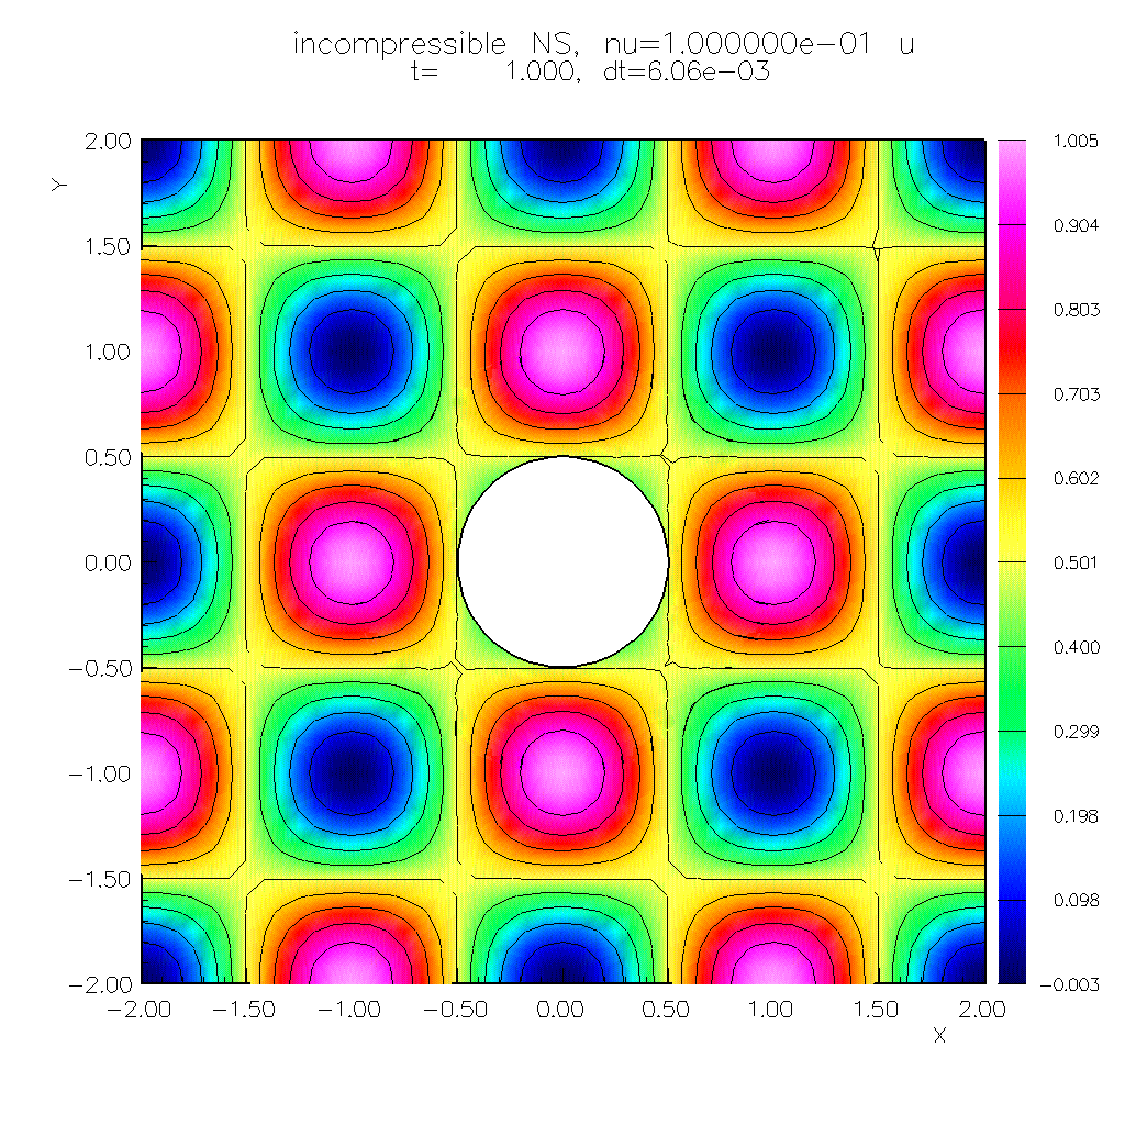
\epsfig{file=\obFigures/ins.cic3.tz.ps,width=.7\linewidth} 
  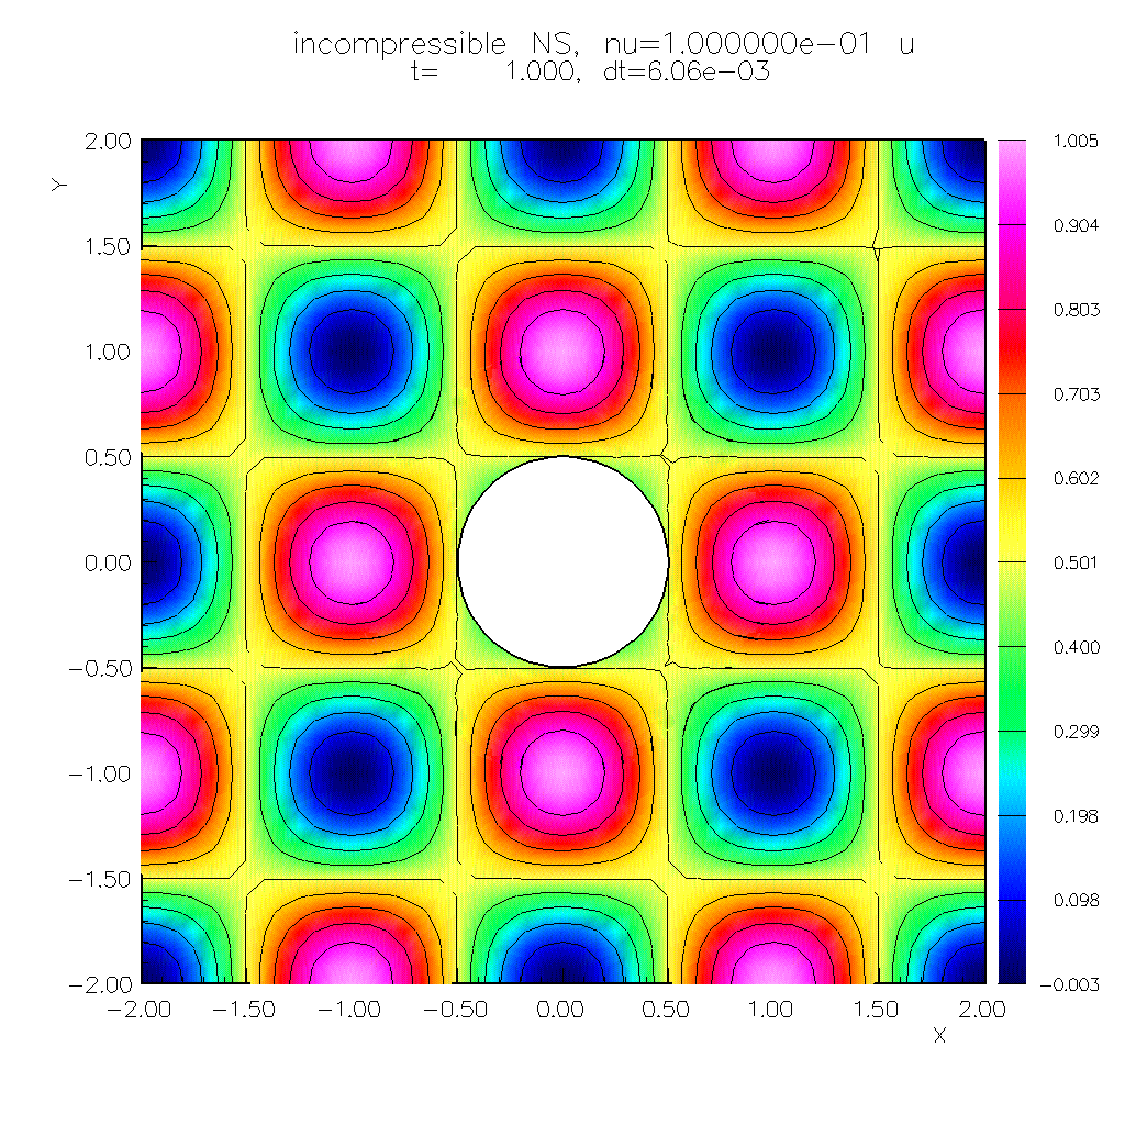
\includegraphics[width=.7\linewidth]{./fig/ins_cic3_tz}
  \caption{Incompressible N-S, twilight zone solution for convergence test} \label{fig:ins.cic.tz}
  \end{center}
\end{figure}

% ==============================================================================================================
\clearpage
\input performanceResults


% ==============================================================================================================
\clearpage
\input sampleSimulations

% ==============================================================================================================
% \clearpage
% \input viscoPlastic/viscoPlasticResults.tex


% -------------------------------------------------------------------------------------------------
\vfill\eject
\bibliography{../common/journalISI,../common/henshaw,../common/henshawPapers}
\bibliographystyle{siam}


\printindex


\end{document}
